\newpage

\section{Разработка структуры системы}

В данном разделе описана структура разрабатываемой системы, а также модули из которых она состоит. Для кажого модуля определяются входные и выходные данные, так же описываестя взаимосвязь моудлей. Кроме того, в разделе рассказывается про готовые технологии, которые используются модулями в процессе своего функционирования.

Разрабатываемая система состоит из 2 модулей, каждый из которых может работать обособленно, при наличии необходимых ресурсов:

\begin{itemize}
	\item модуль для сбора информации;
	\item модуль для обучения нейросети и предсказания интересов.
\end{itemize}

Необходимо сформировать наиболее точное описание разрабатываемого программного обеспечения. Для этого было принято решение о рассмотрении функциональной диаграммы верхнего уровня.
В данном случае в качестве отображения взаимосвязей была выбрана нотация IDEF0. В качестве входных данные для сбора информации (бланк опроса, изображение автомобиля с номером) и данные для предсказания интересов (возраст владельца и модель авто). В качестве субъекта выступает пользователь и вычислительная машина. Управление задается алгоритмами для сбора данных, алгоритм обучения нейросети, алгоритм работы с обученной моделью. К выходным данным относятся датасет, обученная модель и предсказанные интересы.

Контекстная диаграмма IDEF0 представлена на рисунке~\ref{f:main_struct}.

\begin{figure}[h]
	\centering
	\vspace{\toppaddingoffigure}
	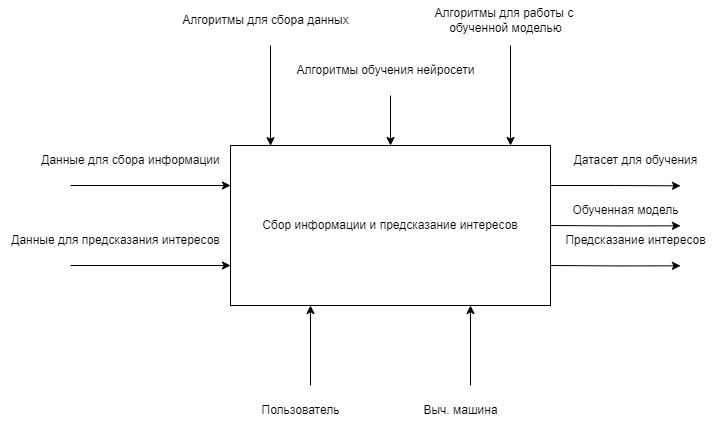
\includegraphics[width=0.6\textwidth]{main_struct}
	\caption{Контекстная диаграмма IDEF0}
	\label{f:main_struct}
\end{figure}

На детализирующей функциональной диаграмме показаны следующие этапы:

\begin{itemize}
	\item сбор информации;
	\item предсказание интересов.
\end{itemize}

Детализированная контекстная диаграмма представлена на рисунке~\ref{f:main_struct_det}

\begin{figure}[h]
	\centering
	\vspace{\toppaddingoffigure}
	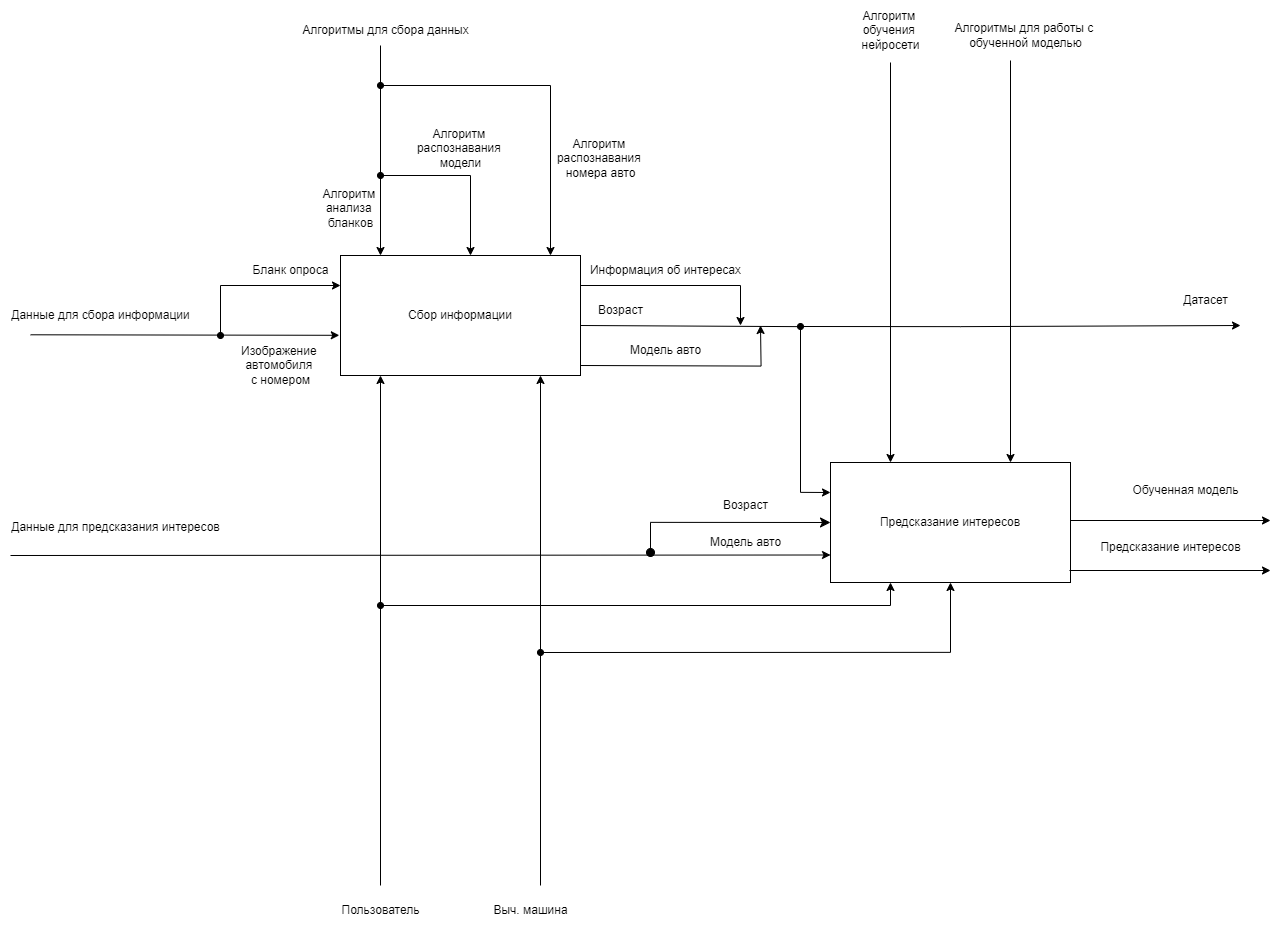
\includegraphics[width=0.8\textwidth]{main_struct_det}
	\caption{Детализированная контекстная диаграмма IDEF0}
	\label{f:main_struct_det}
\end{figure}

Как видно из схемы, разрабатываемая система состоит из 2 модулей: сбора информации и предсказания интересов. Далее рассмотрим каждый из них подробнее.



\subsection{Разработка структуры компонента для сбора информации}

В данном разделе будет детально рассмотрена структура модуля, его функции и алгорритмы функционирования. В разделе описываются компоненты, из которых состоих сам модуль, а так же связь между ними.


\subsubsection{Определение ключевых функций}

Разрабатываемый модуль состоит из трех компонентов. Рассмотрим функционал каждого подробнее.

\paragraph{Сбор и обработка данных}

Модуль должен быть способен автоматически собирать опросные данные с заполненных анкет посетителей парковки.

Был определен ряд вопросов, который позволяют определить некоторые основные интересы:
\begin{itemize}
    \item ­интересуетесь ли вы искусством (картины, скульптура, музыка и т.д.);
    \item ­занимаетесь ли вы спортом или физической активностью;
    \item ­любите ли вы чтение книг или просмотр фильмов;
    \item ­интересуетесь ли вы наукой и технологиями;
    \item ­увлекаетесь ли вы путешествиями и открытием новых мест;
    \item ­является ли для вас кулинария или готовка хобби;
    \item ­интересуетесь ли вы политикой и общественными вопросами.
\end{itemize}

Так же на бланке (представлен на рисунке~\ref{f:blank} выше) присутствует поле, в котором опрашиваемый должен указать свой возраст. 

Опрашиваемый должен закрасить кружки, соответствующие его ответу на каждый вопрос, а также указать свой возраст.

Бланк на вход должен подаваться в виде фотографии или скан копии.

Присутсвует возможность изменить блнак. Вопросы пользователь может выбрать произвольно, главное, чтобы они были представленны в определенном в примере формате. Для изменения областей интересов, с которыми работает система, необходимо внести их списком в текстовый файл. Далее система будет подгружать их в таблицу. Сам файл хранится в папке конфигурации по пути \textbackslash cfg от корневой папки и выглядит следущим образом (пример файла привен на рисунке~\ref{f:file-cfg}).

\begin{figure}[ht]
	\centering
	\vspace{\toppaddingoffigure}
	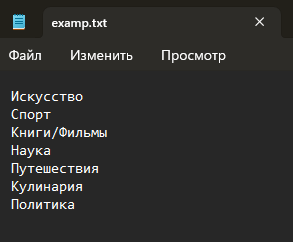
\includegraphics[width=0.45\textwidth]{file-cfg}
	\caption{Пример файла с конфигурацией областей интересов}
	\label{f:file-cfg}
\end{figure}

После сбора данных необходимо провести их предварительную обработку, включая распознавание текста и извлечение ответов на вопросы опроса.


\paragraph{­Распознавание номеров автомобилей}

Модуль должен обеспечивать распознавание номеров автомобилей с изображений, полученных с камер видеонаблюдения на парковке.

Разрешение входного изображения должно быть не ниже 1280х720. Кроме того, распознаваемый номер должен быть читаем, то есть быть чистым, не выцветшим и не закрыт посторонними предметами. Это позволит повысить точность распознавания и сократить количество ошибок.

После распознавания номеров необходимо извлечь информацию о модели автомобиля и ассоциировать её с данными о посетителе.

\paragraph{Поиск модели автомобиля}

Данный модуль должен по распознанному номеру найти модель автомобиля. Данная процедура должна выполнятся с помощью сторонних сервисов, например "Номерограмм.ру", которые позволяют получить базовую информации об автомобиле, на основе WIN-номера или гос. регистрационного знака.



\subsubsection{Структура модуля}

Необходимо сформировать наиболее точное описание разрабатываемого программного обеспечения. Для этого было принято решение о рассмотрении функциональной диаграммы верхнего уровня.

В данном случае в качестве отображения взаимосвязей была выбрана нотация IDEF0. В качестве входных бланк опроса и изображение автомобиля. В качестве субъекта выступает пользователь и вычислительная машина. Управление задается алгоритмами анализа бланков, распознавания номера и получения модели автомобиля. К выходным данным будут относиться информация об интересах посетителя, его возраст и модель машины.
Контекстная диаграмма IDEF0 представлена на рисунке~\ref{f:getdate_struct}.

\begin{figure}[ht]
	\centering
	\vspace{\toppaddingoffigure}
	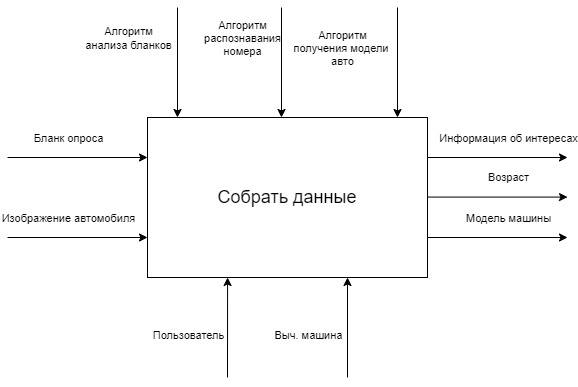
\includegraphics[width=0.7\textwidth]{getdate_struct}
	\caption{Контекстная диаграмма IDEF0}
	\label{f:getdate_struct}
\end{figure}

Детализирующая функциональная диаграмма более подробно раскрывает функциональную диаграмму верхнего уровня: описывает взаимодействия и связи процессов, происходящих внутри системы. На ней можно увидеть, какие процессы взаимосвязаны и что между ними общего.
На детализирующей функциональной диаграмме показаны следующие этапы:

\begin{itemize}
    \item анализ бланков. Входными данными являются бланки опросов. На выход поступает информация об интересах и возраст опрашиваемого;
    \item­ распознавание номеров. Входными данными являются изображения автомобилей. На выход поступает государственный номер автомобиля;
    \item­ определение модели. На вход поступает номер автомобиля, а на выход идет модель машины.
\end{itemize}

Детализированная контекстная диаграмма представлена на рисунке~\ref{f:getdate_struct_det}.
\begin{figure}[ht]
	\centering
	\vspace{\toppaddingoffigure}
	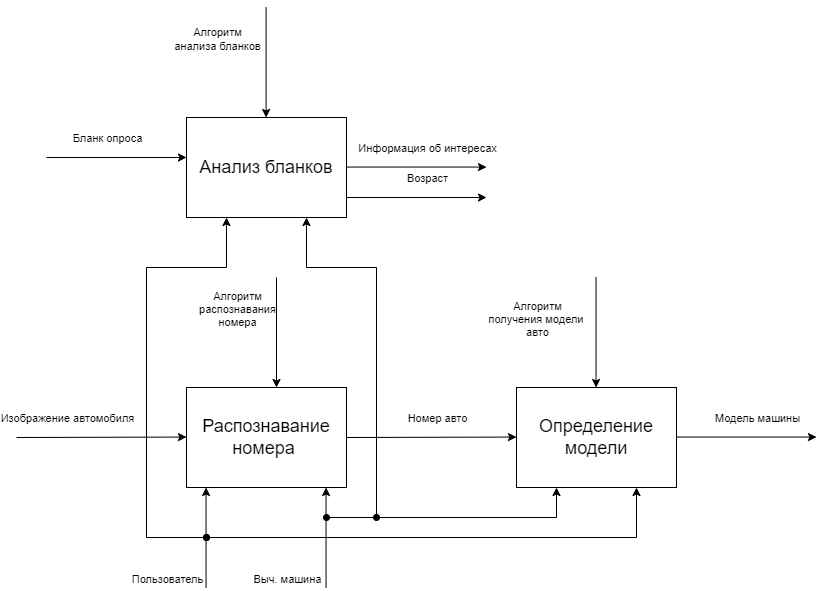
\includegraphics[width=0.7\textwidth]{getdate_struct_det}
	\caption{Детализированная контекстная диаграмма IDEF0}
	\label{f:getdate_struct_det}
\end{figure}

Таким образом, разрабатываемый модуль будет состоять из трех основных компонентов: «Анализ бланков», «Определение модели», «Распознавание номера».

Так же стоит определить формат создаваемого датасета. В него будет входить вся получаемая информация. Следовательно, датасет будет иметь следующие поля:

\begin{itemize}
    \item model: модель автомобиля;
    \item age: возраст;
    \item art: интерес к искусству;
    \item sport: интерес к спорту;
    \item book/film: интерес к фильмам и книгам;
    \item science: интерес к науке и технологиям;
    \item travel: интерес к путешествиям;
    \item cooking: интерес к готовке;
    \item politics: интерес к политике.
\end{itemize}


\subsubsection{Анализатор бланков}

Основными функциями компонента являются функции для анализа анкет, сбора информации об ответах и возрасте, указанном на бланке.

Задача компонента заключается в анализе анкет. Он должен автоматически обрабатывать изображения анкет, извлекать информацию об ответах на вопросы и возрасте, указанном на бланке.

Для выполнения задачи выбраны следующие инструменты:
\begin{itemize}
    \item OpenCV: для обработки изображений, выделения контуров и преобразований перспективы;
    \item imutils: для удобной работы с изображениями, сортировки контуров и других операций;
    \item pytesseract: для распознавания текста на изображениях с использованием технологии OCR.
\end{itemize}

На вход компоненту подается изображение анкеты. Это может быть фотография сверху или скан копия бланка. После своей работы результаты будут сохраняются в CSV-файл.

Рассмотрим алгоритм работы компонента:
\begin{enumerate}
    \item начало: вход в компонент;
    \item ­загрузка изображения: компонент получает на вход изображение анкеты для анализа;
    \item ­препроцессинг изображения;
        \begin{enumerate}
            \item преобразование в оттенки серого;
            \item сглаживание с помощью фильтра Гаусса;
            \item применение оператора Canny для обнаружения границ;
        \end{enumerate}
    \item ­поиск области анкеты;
        \begin{enumerate}
            \item поиск контуров на изображении;
            \item определение контура анкеты;
        \end{enumerate}
    \item выделение области анкеты;
        \begin{enumerate}
            \item применение преобразования перспективы для выделения области анкеты;
            \item получение и сохранение выделенной области;
        \end{enumerate}
    \item обработка анкеты;
        \begin{enumerate}
            \item применение пороговой обработки к выделенной области для получения четкого изображения;
            \item обнаружение контуров на обработанном изображении;
            \item определение контуров блоков с ответами на анкете;
        \end{enumerate}
    \item анализ ответов;
        \begin{enumerate}
            \item идентификация блоков с ответами на анкете;
            \item определение заполненных ответов в каждом блоке;
            \item оценка правильности ответов согласно ключу ответов;
            \item формирование списка результатов анализа;
        \end{enumerate}
    \item извлечение возраста;
        \begin{enumerate}
            \item определение области, содержащей возраст на анкете;
            \item применение преобразования перспективы для выделения области с возрастом;
            \item применение пороговой обработки и распознавание текста для извлечения возраста;
        \end{enumerate}
    \item запись результатов: сохранение результатов анализа и возраста в файл;
    \item конец: завершенеи работы компонента.
\end{enumerate}

Алгоритм работы компонента представлен на рисунке~\ref{f:blank_alg}.
\begin{figure}[ht]
	\centering
	\vspace{\toppaddingoffigure}
	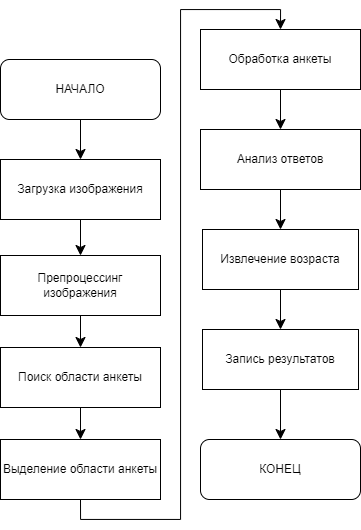
\includegraphics[width=0.4\textwidth]{blank_alg}
	\caption{Алгоритм работы анализатора}
	\label{f:blank_alg}
\end{figure}

Данный модуль в принципе является самостоятельным. Он может использоваться в различных областях, где требуется автоматизированный анализ анкет. Также при желании, его можно расширить и настроить для анализа других типов анкет.

Также не стоит забывать об обработке ошибок. При реализации данного компонента необходимо предусмотреть решение ошибочных ситуаций (неправильное распознавание, неверный формат изображения), которые могут возникать в процессе работы, чтобы обеспечить корректную работу.


\subsubsection{Поиск модели автомобиля}

Разработку компонента стоит начать с определения основной функции: обеспечение автоматизированного доступа к информации о моделях автомобилей. Информацию о модели можно взять с различных сайтов, таких как Nomerogram.ru, Avtocod.ru и другие. Важно учесть, что работа с сайтом будет вестись программно, а значит стоит выбрать сайт не только с самой большой базой автомобилей, но и тот, у которого нет «проверки на робота». Из представленных вариантов, а именно Nomerogram.ru, Avtocod.ru, Autoteka.ru, Avtoproverka.ru, имеющих примерно одинаковую базу автомобилей, все кроме Autoteka.ru имеют так называемую «проверку на робота» (рисунок~\ref{f:check_robot}).

\begin{figure}[ht]
	\centering
	\vspace{\toppaddingoffigure}
	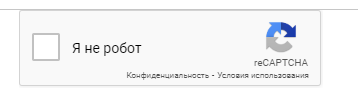
\includegraphics[width=0.4\textwidth]{check_robot}
	\caption{Проверка на робота}
	\label{f:check_robot}
\end{figure}


Следовательно, работа будет происходить именно с Autoteka.ru (рисунок~\ref{f:autoteka}).

\begin{figure}[ht]
	\centering
	\vspace{\toppaddingoffigure}
	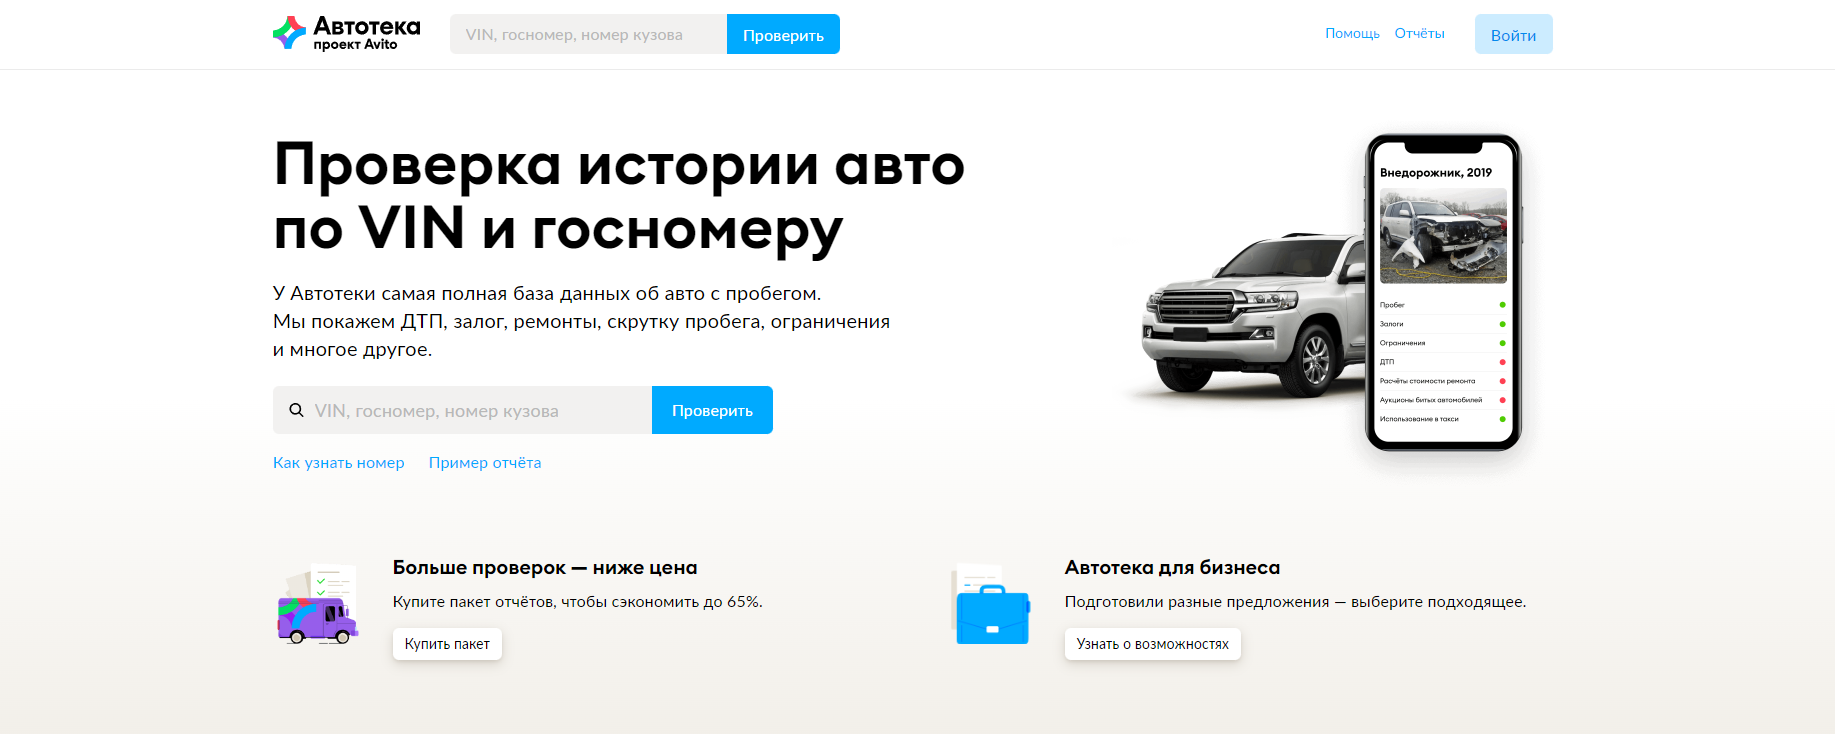
\includegraphics[width=0.85\textwidth]{autoteka}
	\caption{Главный экран Autoteka.ru}
	\label{f:autoteka}
\end{figure}

Autoteka.ru – это веб-сервис, который собирает и предоставляет информацию о различных транспортных средствах на территории России. Он пользуется популярностью среди водителей, автодилеров, страховых компаний и других участников автомобильного сектора. Вот основные характеристики и особенности сайта autoteka.ru:

\begin{itemize}
    \item проверка истории автомобиля. На сайте autoteka.ru пользователи могут проверить историю определенного автомобиля, используя его номер регистрации. Эта функция предоставляет информацию о предыдущих владельцах, результатах технического осмотра, наличии ограничений на регистрацию, участии в ДТП и других значимых данных;
    \item получение технических данных. Люди могут просматривать информацию о технических характеристиках машины, таких как бренд, модель, год выпуска, тип кузова, мощность двигателя и других деталях. Это может быть полезно при принятии решения о покупке или продаже автомобиля;
    \item проверка наличия ограничений. Пользователи имеют возможность проверить, есть ли какие-либо ограничения на регистрацию автомобиля, такие как залоги, аресты или запреты на регистрацию по различным причинам. Это важно для тех, кто планирует приобрести автомобиль, и желает удостовериться в его юридической чистоте перед сделкой;
    \item получение отчетов по автомобилю. Пользователи имеют возможность запросить подробные отчеты об истории автомобиля, включая информацию о предыдущих сделках, количестве владельцев, технических характеристиках, участии в ДТП и прочих данных. Это способствует осознанному выбору при покупке подержанного транспортного средства;
    \item онлайн-консультации. Кроме того, на avtoteka.ru доступны онлайн-консультации и помощь пользователям по вопросам автомобильной истории, юридическим аспектам регистрации транспортных средств и другим темам.
\end{itemize}



Avtoteka.ru – это востребованный ресурс среди пользователей, источник полезной информации о транспортных средствах. С его помощью можно узнать всё, что важно о машине, просто введя VIN-код, госномер или номер кузова. Процесс простой: вводите данные и жмёте "Поиск", после чего получаете страницу с информацией о транспортном средстве (рисунок~\ref{f:autoteka_info}).

\begin{figure}[ht]
	\centering
	\vspace{\toppaddingoffigure}
	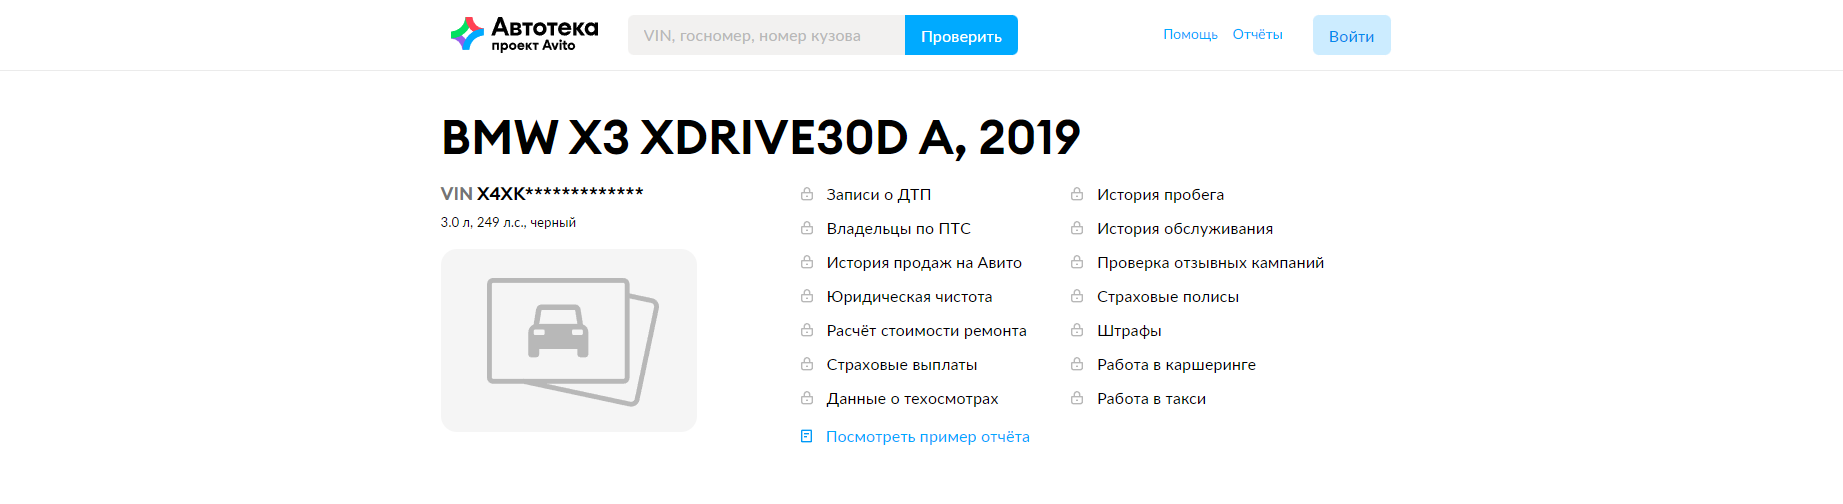
\includegraphics[width=1\textwidth]{autoteka_info}
	\caption{Информация об автомобиле}
	\label{f:autoteka_info}
\end{figure}

Полная информация предоставляется по платной подписке или за разовый платеж, но для выполнения поставленной задачи необходимо получить только модель, что можно сделать бесплатно.


Функциональные требования: компонент должен обеспечивать ввод номера, отправку запроса на сайт Autoteka, получение результатов и извлечение необходимой информации.

Выбор инструментов и технологий: 
\begin{itemize}
    \item для автоматизации взаимодействия с веб-страницами можно использовать библиотеку Selenium для Python, так как она обладает мощными возможностями веб-автоматизации;
    \item для парсинга полученных данных удобно применять инструменты для работы с текстом и регулярные выражения, например, встроенные функции Python.
\end{itemize}


Составление алгоритма работы:
\begin{itemize}
    \item компонент должен открывать веб-браузер, переходить на сайт Autoteka и вводить указанный регистрационный номер;
    \item после получения результата, необходимо обработать страницу с результатами и извлечь нужные данные, такие как модель автомобиля;
    \item важно учесть возможные сценарии ошибок и способы их обработки, например, отсутствие данных по указанному номеру или проблемы с доступом к сайту Autoteka.
\end{itemize}

Алгоритм работы представлен на рисунке~\ref{f:search_alg}.

\begin{figure}[ht]
	\centering
	\vspace{\toppaddingoffigure}
	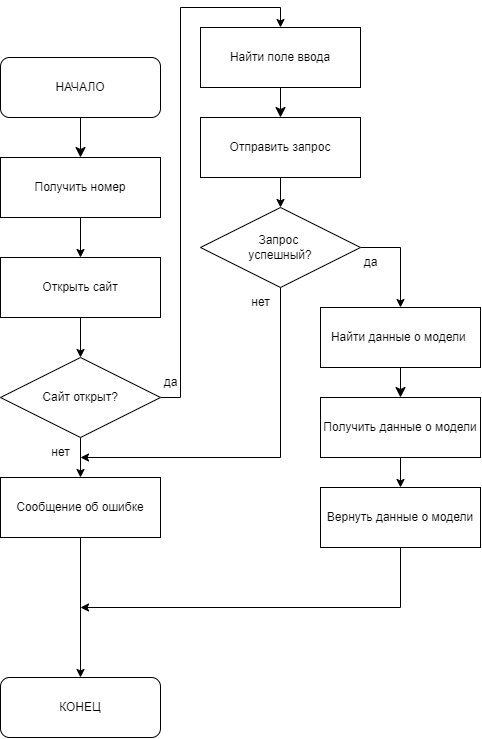
\includegraphics[width=0.5\textwidth]{search_alg}
	\caption{Алгоритм работы компонента для поиска модели}
	\label{f:search_alg}
\end{figure}



\subsubsection{Распознование номера автомобиля}

В этом разделе будет описан компонент, который используется для распознавания номерных знаков автомобиля, его алгоритм и функции. Рвссматриваются модели, которые он использует в процессе своей работы.

\paragraph{Обнаружение положения номерного знака}
Для обнаружения положения номерного знака используется предобученная модель model-resnet.tflite с архитектурой ResNet-50. Она предназначена для выявления границ номерного знака и выделение его области. ResNet-50 выбрана благодаря ее способности эффективно извлекать признаки из изображений и обучаться на больших объемах данных \refref{ref:res-net}. 

ResNet50 состоит из четырех ключевых модулей: сверточные слои, блок идентификации, сверточный блок и полностью связанные слои. Сверточные слои занимаются извлечением признаков из изображений, таких как края, текстуры и формы. Блок идентификации и сверточный блок обрабатывают и преобразовывают эти признаки. В завершение, полностью связанные слои отвечают за финальную классификацию \refref{ref:res-net}.

Сверточные слои ResNet50 состоят из нескольких сверточных блоков, сопровождаемых пакетной нормализацией и активацией. Они извлекают особенности из входных изображений и передают их дальше для анализа. Далее следуют слои объединения, которые уменьшают размеры карт признаков, сохраняя важные детали \refref{ref:res-net}.

Блок идентификации и сверточный блок - это основные строительные блоки ResNet50. Он передает входные данные через ряд сверточных слоев и добавляет к ним остаточные данные. Это позволяет сети изучать функции, оставшиеся после извлечения признаков. Сверточный блок аналогичен блоку идентификации, но использует сверточные слои 1x1 для уменьшения размерности перед основным сверточным слоем 3x3 \refref{ref:res-net}.

Полностью связанные слои выполняют окончательную классификацию. Выходные данные последнего полностью связанного слоя поступают на функцию активации softmax для получения вероятностей классов.

Графическое излбражение структуры представлено на рисунке~\ref{f:res_net}.
\begin{figure}[ht]
	\centering
	\vspace{\toppaddingoffigure}
	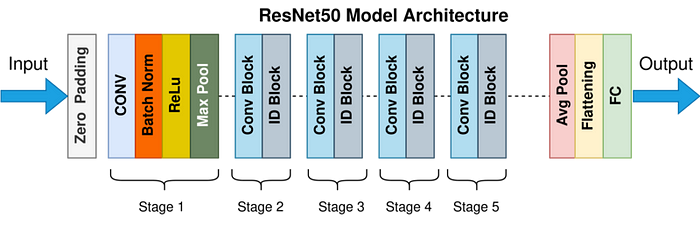
\includegraphics[width=0.7\textwidth]{res_net}
	\caption{Архитектура ResNet-50}
	\label{f:res_net}
\end{figure}



50-уровневая архитектура ResNet включает в себя следующие элементы:

\begin{itemize}
    \item свертка ядра 7 × 7 наряду с 64 другими ядрами с шагом в 2 размера;
    \item максимальный уровень объединения с шагом в 2 размера;
    \item 9 слоев- свертка ядра размером 3 × 3,64, другой с 1 × 1,64 ядрами и третий с 1 × 1256 ядрами. Эти 3 слоя повторяются 3 раза;
    \item 12 слоев с 1 × 1128 ядрами, 3 × 3128 ядрами и 1 × 1512 ядрами, повторяется 4 раза;
    \item 18 слоев с ядрами 1 × 1256 и 2 ядрами 3 × 3,256 и 1 × 1,1024, повторяется 6 раз;
    \item 9 слоев с ядрами 1 × 1512, 3 × 3512 и 1 × 12048 повторяются 3 раза;
    \item создание среднего пула, за которым следует полностью подключенный уровень с 1000 узлами, с использованием функции активации softmax.
\end{itemize}

Тестирование модели показало достаточно хороший уровень точности. Результаты тестирования представлены на рисунке~\ref{f:test1-res-net}.
\begin{figure}[ht]
	\centering
	\vspace{\toppaddingoffigure}
	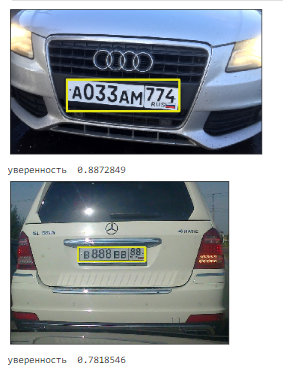
\includegraphics[width=0.3\textwidth]{test1-res-net}
	\caption{Тестирование модели}
	\label{f:test1-res-net}
\end{figure}


\paragraph{Определение номера автомобиля}

Для определения номера автомобиля используется предобученная модель model-nomer.tflite. Данная модель предназначена для определения текста на номерном знаке. фрагмент изображения с номерным знаком поступает от модели, описанной выше. Модель представляет собой комбинацю сверточной нейронной сети (CNN), рекуррентной нейронной сети долгой краткосрочной памяти (LSTM) и функции свертки по времени (CTC) для распознавания текста на изображениях. CNN используется для извлечения признаков из изображения номерного знака, LSTM преобразует эти признаки в последовательность символов, а CTC используется для выравнивания последовательности символов с фактическим текстом номера \refref{ref:cnn-lstm}.

Структура модели представлена на рисунке~\ref{f:cnn-lstm}.

\begin{figure}[h!]
	\centering
	\vspace{\toppaddingoffigure}
	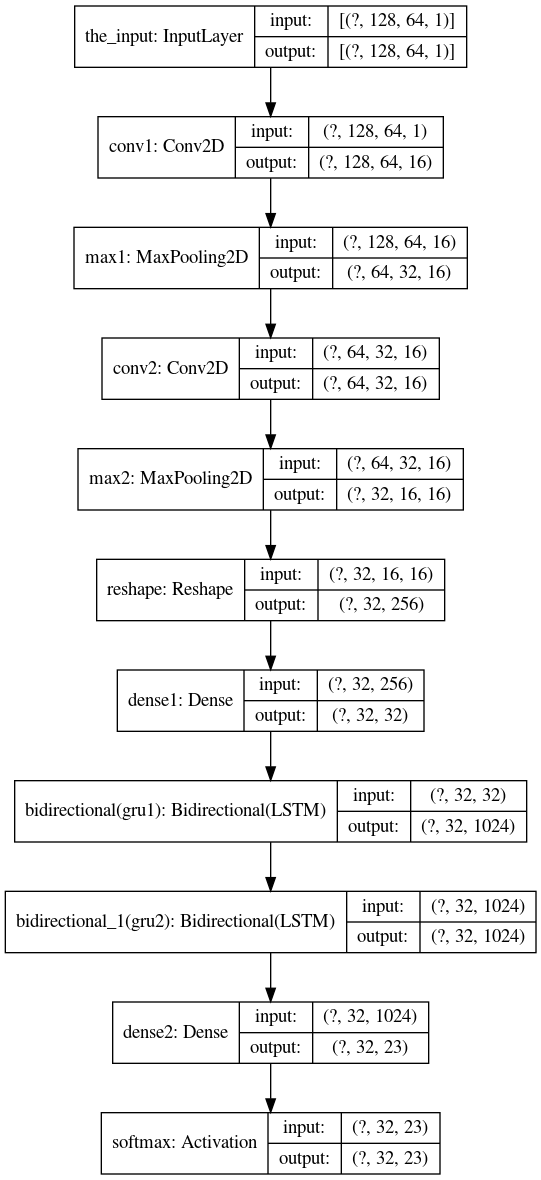
\includegraphics[width=0.4\textwidth]{cnn-lstm}
	\caption{Структура модели}
	\label{f:cnn-lstm}
\end{figure}

Результаты тестирования представлены на рисунке~\ref{f:test-cnn-lstm}.

\begin{figure}[h!]
	\centering
	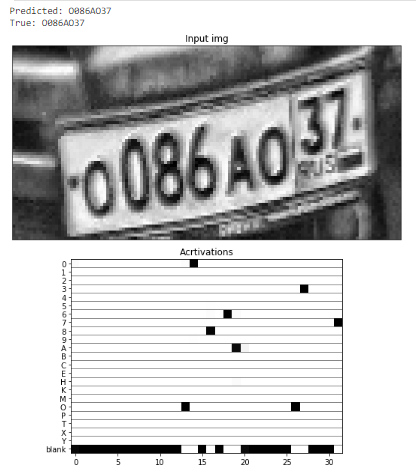
\includegraphics[width=0.4\textwidth]{test-cnn-lstm}
	\caption{Результаты тестирования}
	\label{f:test-cnn-lstm}
\end{figure}

\newpage

\paragraph{Алгоритм компонента}

К функциям компонента относятся следующие пункты:
\begin{itemize}
    \item загрузка и разбиение входного видео на кадры;
    \item выбор отдельного кадра;
    \item распознавание номера автомобиля на получившимся изображении.
\end{itemize}

Алгоритмы работы представлены на рисунках~\ref{f:nomer-alg-main}-~\ref{f:nomer-alg-recognize}.

\begin{figure}[h!]
	\centering
	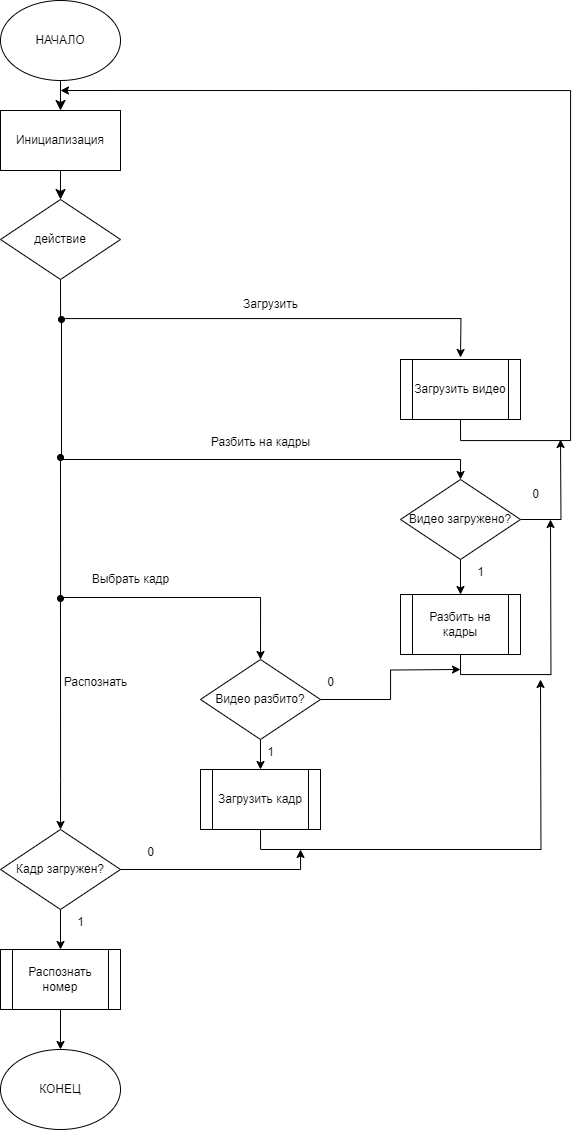
\includegraphics[width=0.6\textwidth]{nomer-alg-main}
	\caption{Схема алгоритма компонента распознавания номера}
	\label{f:nomer-alg-main}
\end{figure}

\newpage
\begin{figure}[h!]
	\centering
	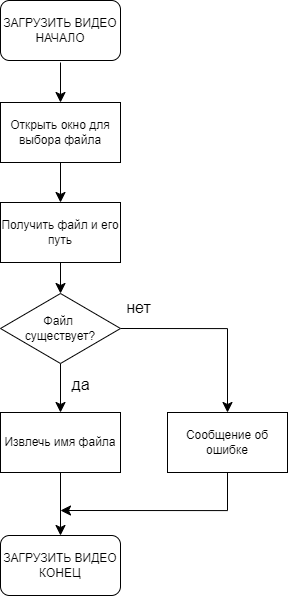
\includegraphics[width=0.22\textwidth]{nomer-alg-load}
	\caption{Схема алгоритма загрузки видео}
	\label{f:nomer-alg-load}
\end{figure}

\begin{figure}[h!]
	\centering
	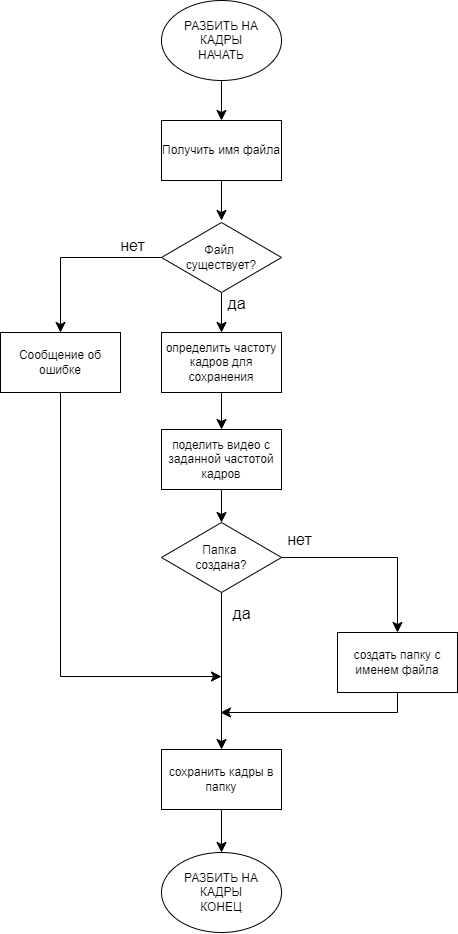
\includegraphics[width=0.35\textwidth]{nomer-alg-split}
	\caption{Схема алгоритма разбиения видео на кадры}
	\label{f:nomer-alg-split}
\end{figure}

\newpage

\begin{figure}[h!]
	\centering
	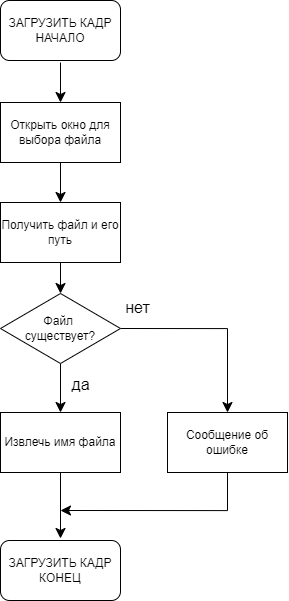
\includegraphics[width=0.22\textwidth]{nomer-alg-choose}
	\caption{Схема алгоритма выбора одного из кадров}
	\label{f:nomer-alg-choose}
\end{figure}

\begin{figure}[h!]
	\centering
	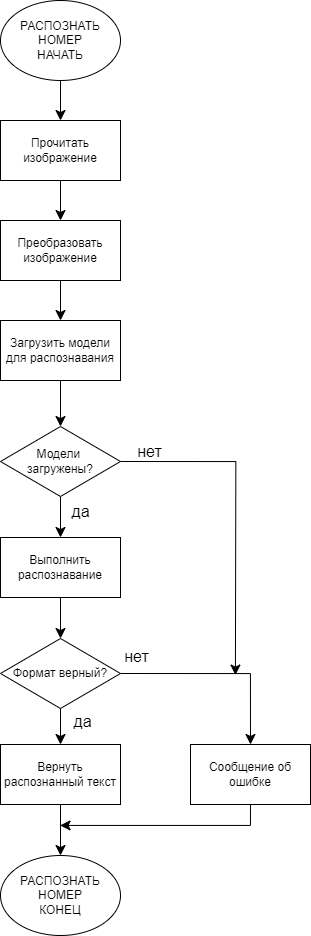
\includegraphics[width=0.25\textwidth]{nomer-alg-recognize}
	\caption{Схема алгоритма распознавания номера}
	\label{f:nomer-alg-recognize}
\end{figure}

\newpage
\section*{Выводы}

В этом разделе было рассмотрено описание модуля для сбора данных, был рассмотрен процесс разработки компонентов, входящих в модуль, а также их функции и особенности.

\subsection{Разработка структуры компонента для обучения нейросети и предсказания интересов}

В данном разделе будет детально рассмотрена структура модуля, его функции и алгоритмы функционирования. Кроме того, будут рассмотрены наиболее популярные методы предсказания, будет обоснован выбор наиболее  


\subsubsection{Определение ключевых функций}

Разрабатываемый модуль должен предсказывать интересы людей на основе их автомобиля и возраста. Интересы разбиваются на различные группы, например:

\begin{itemize}
    \item искусство;
    \item спорт;
    \item книги/фильмы;
    \item наука;
    \item путешествия;
    \item кулинария;
    \item политика.
\end{itemize}

Модуль должен предсказать вероятность того, есть ли у клиента интересы в этих областях, например, 10\% - искусство, 78\% - спорт и так далее.

Для определения разделения на области интересов могут использоваться любые вопросы, то есть можно учитывать интересы людей, относящиеся к другим областям, например, музыка, животные и т.п.

При проектировании модуля для примера используется распределение, который было определено при проектировании модуля, направленног на сбор данных. Ниже приведен список вопросов, которые там применялись:
\begin{itemize}
    \item интересуетесь ли вы искусством (картины, скульптура, музыка и т.д.);
    \item занимаетесь ли вы спортом или физической активностью;
    \item любите ли вы чтение книг или просмотр фильмов;
    \item интересуетесь ли вы наукой и технологиями;
    \item увлекаетесь ли вы путешествиями и открытием новых мест;
    \item является ли для вас кулинария или готовка хобби;
    \item интересуетесь ли вы политикой и общественными вопросами;
    \item так же на бланке присутствует поле, в котором опрашиваемый должен указать свой возраст.
\end{itemize}

Точность предсказания должна быть не ниже 80\%.

\subsubsection{Выбор метода}

В этом разделе будут описаны наиболее популярные методы, которые используются для предсказания чего-либо, а также будет обоснован выбор наиболее подходящего.

\paragraph{Описание искусственных нейронных сетей}

Человеческий мозг великолепно справляется с задачами по распознаванию образов, опережая в этом даже самые передовые компьютеры. Это объясняется особенностями обработки информации в мозге, которые значительно отличаются от методов, используемых в цифровых устройствах. Мозг человека - это сложная, нелинейная и параллельная система обработки данных. Он умело организовывает свои структурные компоненты для успешного решения разнообразных задач, таких как распознавание образов, превосходя при этом даже самые мощные компьютеры в скорости обработки информации \refref{ref:neuron}.

Искусственная нейронная сеть – это сложный параллельный процессор, который состоит из множества элементарных блоков, называемых нейронами, предназначенных для обработки информации. Эти нейроны накапливают опыт и передают его для дальнейшей обработки \refref{ref:neuron}.

Ниже приведены некоторые преимущества нейронных сетей:
\begin{itemize}
    \item нелинейность, что позволяет моделировать сложные отношения в данных;
    \item преобразование входящей информации в выходные результаты;
    \item адаптивность, позволяющая сети настраиваться под различные задачи;
    \item понятность ответов, делая выводы из сети более интерпретируемыми;
    \item учёт контекстной информации для более точных прогнозов;
    \item способность к отказоустойчивости, что позволяет сохранять работоспособность даже при некоторых повреждениях;
    \item единообразный подход к анализу и проектированию.
\end{itemize}


Обучение нейронной сети, или ее настройка, представляет собой процесс изменения свободных параметров сети через моделирование ее взаимодействия с окружающей средой. Тип обучения определяется выбором метода для определения характеристик.

Этот процесс настройки можно описать следующей последовательностью действий:
\begin{enumerate}
    \item cеть получает стимулы извне;
    \item свободные параметры сети подвергаются изменениям;
    \item после изменений во внутренней структуре нейронная сеть реагирует на входные стимулы по-новому.
\end{enumerate}

Алгоритм обратного распространения, известный как один из основных методов обучения, находит свое место среди разнообразных алгоритмов обучения. Наиболее известным и широко применяемым из них является алгоритм обратного распространения. Этот метод нацелен на минимизацию разницы между реальными выходными значениями нейронной сети (ANN) и желаемыми выходами. Его детальное описание можно найти в источниках \refref{ref:back-error}.

Суть обучения через алгоритм обратного распространения заключается в переводе задачи отображения от входных данных к выходным значениям (путем использования набора примеров) в установку оптимальных синаптических весов и порогов для многослойного персептрона. Процесс настройки сети можно рассматривать как выбор наилучшей модели из набора "кандидатов" структур, основанный на определенных критериях \refref{ref:back-error}.

\begin{figure}[h!]
    \centering
    \vspace{\toppaddingoffigure}
    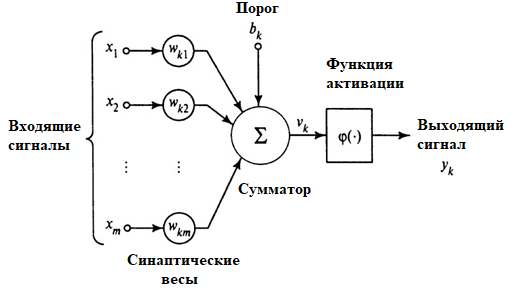
\includegraphics[width=0.7\textwidth]{neuron}
    \caption{Нелинейная модель нейрона}
    \label{f:neuron}
\end{figure}

Нейрон, в контексте нейронных сетей, представляет собой ключевую единицу обработки информации \refref{ref:neuron-model}. На рисунке~\ref{f:neuron} представлена модель нейрона, которая лежит в основе искусственных нейронных сетей. Эта модель включает в себя три основных компонента.

Ансамбль синапсов состоит из множества связей, каждая из которых имеет свой собственный вес или силу. Сумматор суммирует входные сигналы, учитывая их веса, которые связаны с соответствующими синапсами нейрона. Функция активации контролирует выходной сигнал нейрона, ограничивая его амплитуду \refref{ref:neuron-model}.

Модель нейрона также может включать пороговый элемент, обозначаемый символом  $b_k$, который влияет на функцию активации, регулируя входной сигнал.

Математически, работу нейрона можно описать следующими уравнениями

\begin{gather}
    u_k = \displaystyle\sum_{j=1}^{m} w_{kj} * x_j, \\
    y_k = \phi * (u_k + b_k)
\end{gather}

где $x_1, x_2, ... , x_m$ - входные сигналы 

$w_{k1}, w_{k2}, ... , w_{km}$ - синаптические весы нейрона $k$

$u_k$ - линейная комбинация входных действий (выход линейного комбинатора)

$b_k$- порог; $\phi()$ – функция активации

$y_k$ является выходным сигналом нейрона.

Постсинаптический потенциал рассчитывается следующим образом
\begin{gather}
    v_k = u_k + b_k
\end{gather}

Функции активации - это особые инструменты, которые определяют, какой будет выходной сигнал нейрона в ответ на воздействие на него окружающей области. Давайте рассмотрим несколько различных функций активации. Кроме перечисленных, существует еще множество других функций активации \refref{ref:neuron-model}.

Одной из таких функций является сигмовидная функция. Она примечательна тем, что быстро переходит от линейного к нелинейному поведению. Логистическая функция является примером сигмовидной функции и может быть представлена следующим образом
\begin{gather}
    f(x) = \frac{1}{1 + e^{-x}}
\end{gather}

\paragraph{Наивный байесовский классификатор}

Наивный байесовский классификатор (Naive Bayes classifier) – это вероятностный алгоритм, основанный на теореме Байеса. Он делает строгое (наивное) предположение о том, что признаки независимы друг от друга для каждого заданного класса. Это предположение значительно упрощает процесс классификации, так как позволяет оценивать одномерные вероятностные плотности вместо многомерных \refref{ref:nbc}.

В этом контексте одномерная вероятностная плотность означает оценку вероятности каждого отдельного признака при условии их независимости, тогда как многомерная плотность оценивает вероятность комбинации всех признаков, предполагая их взаимозависимость. Классификатор называется наивным именно потому, что такое предположение значительно упрощает вычисления и улучшает эффективность алгоритма. Однако, на практике, предположение о независимости признаков часто не соответствует действительности, что может существенно снизить качество прогнозов в некоторых случаях \refref{ref:nbc}.

Сама же формула Байеса выглядит следующим образом
\begin{gather}
    P(A|B) = \frac{P(B|A) * P(A)}{P(B)}
\end{gather}

где $P(A|B)$ — апостериорная вероятность события A при условии выполнения события B

$P(B|A)$ — условная вероятность события B при условии выполнения события A

$P(A)$ и $P(B)$ — априорные вероятности событий A и B соответственно.

% \begin{itemize}
%     \item $P(A|B)$ — апостериорная вероятность события A при условии выполнения события B;
%     \item $P(B|A)$ — условная вероятность события B при условии выполнения события A;
%     \item $P(A)$ и $P(B)$ — априорные вероятности событий A и B соответственно.
% \end{itemize}

А в контексте машинного обучения формула Байеса приобретает следующий вид
\begin{gather}
    P(y_k|X) = \frac{P(X|y_k) * P(y_k)}{P(X)}
\end{gather}

где $P(yk|X)$ — апостериорная вероятность принадлежности образца к классу $y_k$ с учётом его признаков X

$P(X|yk)$ — правдоподобие, то есть вероятность признаков X при заданном классе $y_k$

$P(yk)$ — априорная вероятность принадлежности случайно выбранного наблюдения к классу $y_k$

$P(X)$ — априорная вероятность признаков X.


% \begin{itemize}
%     \item $P(yk|X)$ — апостериорная вероятность принадлежности образца к классу $y_k$ с учётом его признаков X;
%     \item $P(X|yk)$ — правдоподобие, то есть вероятность признаков X при заданном классе $y_k$;
%     \item $P(yk)$ — априорная вероятность принадлежности случайно выбранного наблюдения к классу $y_k$;
%     \item $P(X)$ — априорная вероятность признаков X.
% \end{itemize}

Если объект описывается не одним, а несколькими признаками $X_1, X_2, ... , X_n$, то формула принимает вид

\begin{gather}
    P(y_k|X_1, X_2, ... , X_n) = \frac{P(y_k) * \displaystyle\prod_{i=1}^{n}{P(X_i|y_k)}}{P(X_1, X_2, ... , X_n)}
\end{gather}


На практике основное внимание уделяется числителю формулы, так как знаменатель зависит только от признаков и не влияет на класс. Поэтому его часто опускают при сравнении вероятностей различных классов. В результате правило классификации сводится к выбору класса с максимальной апостериорной вероятностью.

\begin{gather}
    y_k \propto arg max P(y_k) \displaystyle\prod_{i=1}^{n}{P(X_i|y_k)}
\end{gather}

Для оценки параметров модели, то есть вероятностей $P(y_k)$ и $P(X_i|y_k)$, обычно применяется метод максимального правдоподобия, который в данном случае основан на частотах встречаемости классов и признаков в обучающей выборке.



\paragraph{Логистическая регрессия}

Логистическая регрессия – это метод анализа данных, который применяет математические методы для выявления взаимосвязей между двумя переменными. Эти взаимосвязи затем используются для прогнозирования значения одной переменной на основе другой. Обычно результаты прогноза имеют ограниченное количество возможных исходов, например, "да" или "нет" \refref{ref:log-reg}.

Модель логистической регрессии имеет несколько составляющих:
\begin{itemize}
    \item уравнения. В математике уравнения выражают зависимость между двумя переменными, например, $x$ и $y$. Эти уравнения позволяют построить график по осям $x$ и $y$, подставляя различные значения $x$ и $y$. Например, если построить график для уравнения $y = 2 * x$, получится прямая линия. Поэтому такие уравнения называют линейными \refref{ref:log-reg};
    \item переменные. В статистике переменные – это факторы или атрибуты данных, значения которых могут изменяться. В анализе некоторые переменные являются независимыми или объясняющими и служат причиной результата. Другие переменные зависят от первых и называются зависимыми переменными или переменными отклика. Логистическая регрессия исследует, как независимые переменные влияют на зависимую, анализируя их исторические значения. В нашем примере x является независимой переменной, предиктором или объясняющей переменной, потому что ее значение известно. А y является зависимой переменной, результатом или переменной отклика, так как ее значение необходимо предсказать \refref{ref:log-reg};
    \item функция логистической переменной. Логистическая регрессия – это статистическая модель, использующая логистическую или логит-функцию в качестве уравнения между $x$ и $y$. Логит-функция отображает y как сигмоидальную функцию от $x$ \refref{ref:log-reg}.
\end{itemize}

\paragraph{Обоснование выбора метода}

Ниже приведены достоинства и недостатки рассмотренных методов.

Плюсы логистической регрессии:
\begin{itemize}
    \item простота реализации и интерпретации;
    \item эффективность при линейной разделяющей гиперплоскости;
    \item меньшая склонность к переобучению на небольших наборах данных;
    \item хорошо работает с линейно разделимыми данными.
\end{itemize}

Минусы логистической регрессии:
\begin{itemize}
    \item ограничение на моделирование нелинейных зависимостей;
    \item ограниченная способность к обработке больших объемов данных;
    \item не учитывает взаимосвязи между признаками.
\end{itemize}


Плюсы наивного байесовского классификатора:
\begin{itemize}
    \item простота и скорость обучения;
    \item эффективность на небольших наборах данных;
    \item меньшая склонность к переобучению.
\end{itemize}

Минусы наивного байесовского классификатора:
\begin{itemize}
    \item предположение о независимости признаков может быть слишком сильным и нереалистичным;
    \item не способен улавливать сложные взаимосвязи между признаками;
    \item требует хорошо подготовленных данных.
\end{itemize}

Плюсы нейронных сетей:
\begin{itemize}
    \item способность моделировать сложные нелинейные зависимости;
    \item автоматическое извлечение признаков из данных;
    \item гибкость и адаптивность к различным типам данных и задачам;
    \item эффективность на больших объемах данных;
    \item улучшенная производительность на сложных задачах.
\end{itemize}

Минусы нейронных сетей:
\begin{itemize}
    \item требуют большого объема данных для обучения;
    \item сложность интерпретации модели;
    \item большое количество настраиваемых параметров, требующих подбора.
\end{itemize}

Исходя из приведенного выше анализа, нейронные сети выделяются среди других методов машинного обучения благодаря их способности моделировать сложные зависимости и обрабатывать большие объемы данных.

% \subsubsection{Проектирование модуля}

\subsubsection{Структура модуля}

Необходимо сформировать наиболее точное описание разрабатываемого программного обеспечения. Для этого было принято решение о рассмотрении функциональной диаграммы верхнего уровня.

В данном случае в качестве отображения взаимосвязей была выбрана нотация IDEF0. В качестве входов датасет для обучения нейросети, возраст посетителя, модель автомобиля посетителя. В качестве субъекта выступает пользователь и вычислительная машина. Управление задается алгоритмами обучения нейронной сети и алгоритмом работы с обученной моделью. К выходным данным будут относиться предсказанные интересы посетителя.

Контекстная диаграмма IDEF0 представлена на рисунке~\ref{f:neuro-struct}

\begin{figure}[h!]
    \centering
    \vspace{\toppaddingoffigure}
    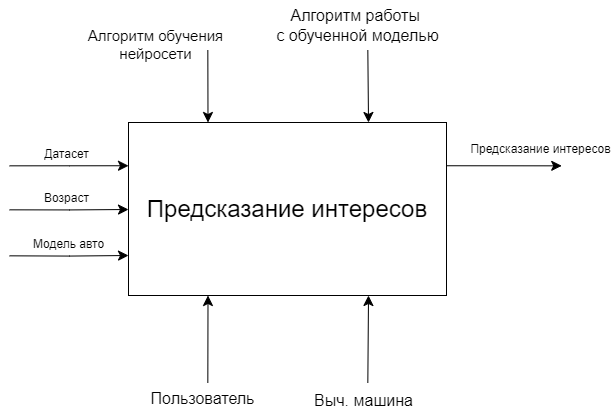
\includegraphics[width=0.5\textwidth]{neuro-struct}
    \caption{Контекстная диаграмма IDEF0}
    \label{f:neuro-struct}
\end{figure}

Детализирующая функциональная диаграмма более подробно раскрывает функциональную диаграмму верхнего уровня: описывает взаимодействия и связи процессов, происходящих внутри системы. На ней можно увидеть, какие процессы взаимосвязаны и что между ними общего.

На детализирующей функциональной диаграмме показаны следующие этапы:
\begin{itemize}
    \item обучение нейросети. На вход поступает датасет, а на выходе получается обученная модель;
    \item определение интересов. На вход поступает обученная модель, а на выход предсказанные интересы.
\end{itemize}

Детализированная контекстная диаграмма представлена на рисунке~\ref{f:neuro-struct-det}

\begin{figure}[h!]
    \centering
    \vspace{\toppaddingoffigure}
    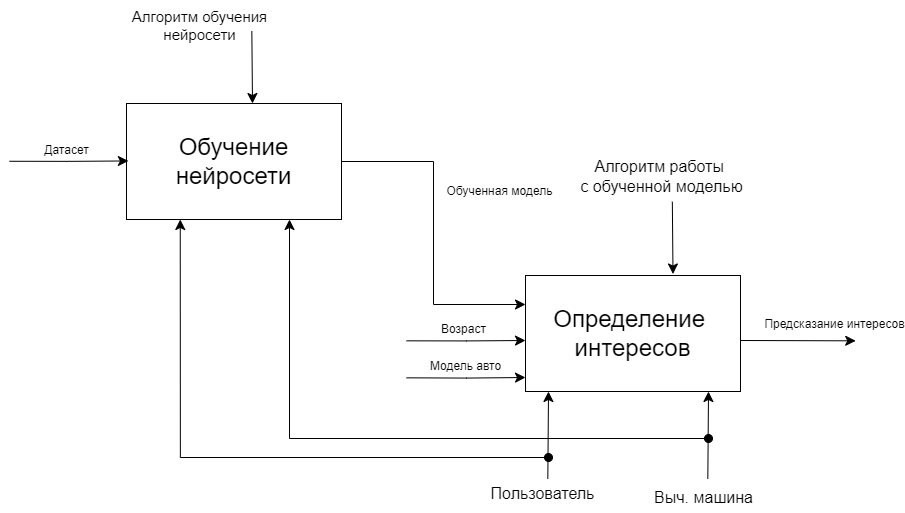
\includegraphics[width=0.8\textwidth]{neuro-struct-det}
    \caption{Детализированная контекстная диаграмма IDEF0}
    \label{f:neuro-struct-det}
\end{figure}

Таким образом, разрабатываемый модуль будет состоять из двух основных компонентов: «Обучения нейросети», «Определение интересов».

% Так же стоит определить формат датасета, который используется для обучения нейросети. В него входит вся информация, которую можно получить с помощью описанного выше модуля для сбора данных. Следовательно, датасет имеет следующие поля:

% \begin{itemize}
%     \item model: модель автомобиля;
%     \item age: возраст;
%     \item art: интерес к искусству;
%     \item sport: интерес к спорту;
%     \item book/film: интерес к фильмам и книгам;
%     \item science: интерес к науке и технологиям;
%     \item travel: интерес к путешествиям;
%     \item cooking: интерес к готовке;
%     \item politics: интерес к политике.
% \end{itemize}


\subsubsection{Алгоритм обучения нейронной сети}

В этом разделе рассматривается общий алгоритм обучения нейронных сетей, который включает в себя загрузку, предварительную обработку и разделение данных, определение архитектуры модели, обучение, оценку производительности и настройку гиперпараметров. Понимание этого алгоритма позволит лучше понять процесс создания и настройки нейронных сетей для решения конкретных задач машинного обучения. Сам алгоритм представлен на рисунке~\ref{f:neuro-learn}

\begin{figure}[h!]
    \centering
    \vspace{\toppaddingoffigure}
    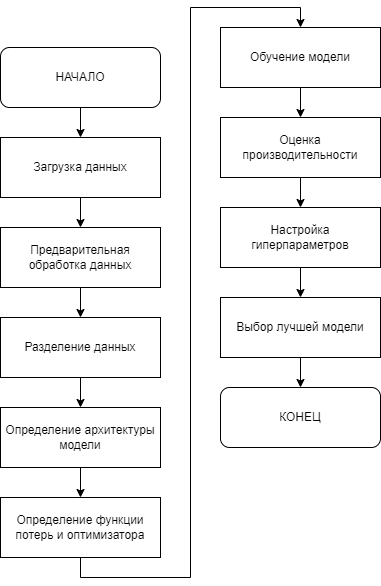
\includegraphics[width=0.5\textwidth]{neuro-learn}
    \caption{Алгоритм обучения сети}
    \label{f:neuro-learn}
\end{figure}

Рассмотрим алгоритм подробнее:
\begin{enumerate}
    \item загрузка данных. Начинаем с загрузки данных из источника, чаще всего из файлов CSV, баз данных или других источников данных;
    \item предварительная обработка данных. Перед тем как данные попадут в модель, их необходимо подготовить. Это может включать в себя удаление или заполнение отсутствующих значений, преобразование категориальных переменных в числовые (например, с помощью кодирования One-Hot), нормализацию числовых данных и т.д.;
    \item разделение данных. Для оценки модели данные обычно разделяются на обучающий и тестовый наборы. Обучающий набор используется для обучения модели, а тестовый - для оценки ее производительности;
    \item определение архитектуры модели. Решается, какая будет архитектура нейронной сети: сколько слоев и скрытых нейронов в каждом слое, какие функции активации использовать, будет ли применяться метод регуляризации (например, Dropout), и т.д.;
    \item определение функции потерь и оптимизатор. Выбирается функция потерь (например, кросс-энтропия для классификации) и оптимизатор (например, стохастический градиентный спуск, Adam и т.д.), которые будут использоваться в процессе обучения;
    \item обучение модели. Модель обучается на обучающем наборе данных. Обычно это включает в себя несколько эпох обучения, где каждая эпоха представляет собой один проход по всем обучающим данным;
    \item оценка производительности модели. После завершения обучения модель оценивается на тестовом наборе данных, чтобы определить ее производительность и обобщающую способность;
    \item настройка гиперпараметров. Для улучшения производительности модели может быть выполнен подбор оптимальных гиперпараметров, таких как количество слоев, количество нейронов, скорость обучения и т.д.;
    \item выбор лучшей модели. Выбирается модель с лучшей производительностью на основе метрик оценки, таких как точность (accuracy), F1-мера, и т.д.;
    \item интеграция с обратной связью. Для улучшения обучения и производительности модели могут быть применены различные методы обратной связи, такие как ранняя остановка (Early Stopping), адаптивная скорость обучения и т.д.
\end{enumerate}


\subsubsection{Описаение структуры нейронной сети}

Определение структуры нейронной сети включает в себя выбор архитектуры сети, составление слоев и их параметров. Обычно структура нейронной сети определяется в соответствии с характеристиками входных данных, задачей, которую необходимо решить, и требованиями к производительности и точности.

В данном случае, для решения задачи многоклассовой классификации, используется последовательная модель нейронной сети, что означает, что слои нейронов последовательно соединены друг с другом. Вот общая структура нейронной сети:
\begin{enumerate}
    \item входной слой. Входной слой представляет собой первый слой нейронной сети, который принимает входные данные. В данном случае, размерность входного слоя определяется количеством признаков в данных;
    \item скрытые слои. Скрытые слои представляют собой слои нейронов, которые выполняют преобразование входных данных. Каждый скрытый слой состоит из нескольких нейронов (узлов), количество которых определяется архитектурой сети. Для каждого нейрона в скрытом слое применяется активационная функция (например, ReLU) для введения нелинейности и извлечения признаков из входных данных;
    \item выходной слой. Выходной слой представляет собой последний слой нейронной сети, который генерирует выходные данные. В данном случае, выходной слой имеет 7 нейронов, по одному для каждого класса (интереса). Каждый нейрон выходного слоя возвращает вероятность принадлежности к соответствующему классу, что достигается использованием активационной функции сигмоида;
    \item регуляризация. Не стоит забывать о слоях «отсеивания» Dropout, которые помогают предотвратить переобучение путем случайного «выключения» нейронов во время обучения.
\end{enumerate}

Таким образом, структура нейронной сети определяется количеством слоев, количеством нейронов в каждом слое, выбором активационной функции и применением регуляризации для обеспечения лучшей обобщающей способности модели.

Для получения множества моделей с различной архитектурой используют специальные библиотеки-тюнеры, которые по заданным гиперпараметрам для каждого варианта обучают получившуюся сеть, после чего можно выбрать архитектуру сети, показавшую наибольшую точность.

Были выделены следующие параметры, которые учитывались при создании структуры нейронной сети:
\begin{itemize}
    \item num-hidden-layers – число скрытых слоев;
    \item num-neurons – число нейронов в слоях;
    \item activation – функция активации;
    \item dropout-rate – значение слоя Dropout;
    \item optimizer – определяет оптимизатор;
    \item learning-rate – скорость обучения.
\end{itemize}

Разработка нейронной сети производилась на языке Python с использованием библиотеки Keras. Для автоматического подбора параметров использовалась библиотека GridSearchCV.

Лучшие модели имеюют сходные параметры. После проведения эксперементов, было выявлено, что все они имеют по 3 скрытых слоя, одинаковую функцию активации ReLU, оптимизвтор и скорость обучения. Отличными параметрами являются число нейронов, которое у всех моделей разное, и значение слоя отсеивания, которое одинаково и равно 0,2 у 1 и 3 модели, а у 2 модели оно принимает значение 0,1. 

В таблице \ref{t:stat} представлен результат моделей.

% \begin{table}[h!]
%     \Large
%     \begin{threeparttable}
%         \caption{Результат модели}
%         \label{t:stat}
%         \centering
%         \begin{tabularx}{\textwidth}{|>{\centering\arraybackslash}X|>{\centering\arraybackslash}X|}
%             \hline
%             Точность & Ошибка \\
%             \hline
%             0,896    & 0,117  \\
%             \hline
%         \end{tabularx}
%     \end{threeparttable}
%     \vspace{\bottompaddingoftable}
% \end{table}

\begin{table}[h!]
    \Large
    \begin{threeparttable}
        \caption{Результат моделей}
        \label{t:stat}
        \centering
        \begin{tabularx}{\textwidth}{|>{\centering\arraybackslash}X|>{\centering\arraybackslash}X|>{\centering\arraybackslash}X|>{\centering\arraybackslash}X|}
            \hline
            Метрики \textbackslash Модели   &   Модель 1            &   Модель 2            &   Модель 3            \\
            \hline
            Параметры                       &   1-20, 2-20, 3-20    &   1-35, 2-30, 3-20    &  1-30, 2-20, 3-25     \\
            \hline
            Точность                        &   0,869               &   0,834               &   0,823               \\
            \hline
            Ошибка                          &   0,117               &   0,130               &   0,174               \\
            \hline   
        \end{tabularx}
    \end{threeparttable}
    \vspace{\bottompaddingoftable}
\end{table}



На рисунке~\ref{f:ns} представлена структура лучшей модели.



\begin{figure}[h!t]
    \centering
    \vspace{\toppaddingoffigure}
    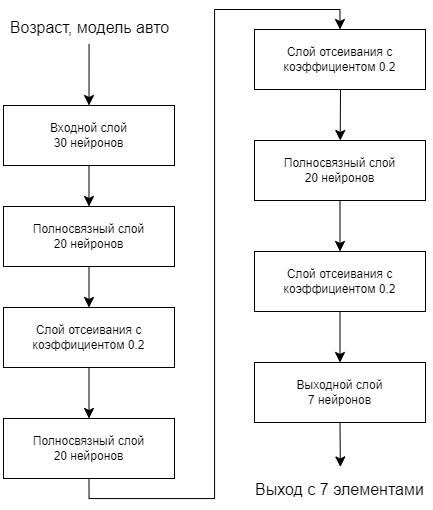
\includegraphics[width=0.45\textwidth]{ns}
    \caption{Структура нейронной сети}
    \label{f:ns}
\end{figure}

\newpage

Из рисунка~\ref{f:ns} видно, что полученная модель состоит из:
\begin{itemize}
    \item входного слоя с 30 нейронами;
    \item 3-х полносвязных слоев с 20 нейронами;
    \item 3 слоев Dropout с коэффициентом 0.2;
    \item выходного слоя с 7 нейронами.
\end{itemize}
Полносвязные и Dropout слои чередуются.

\subsubsection{Разработка модуля}

Основной модуль должен получить от пользователя информацию о модели автомобиля и возрасте владельца. На основе этих данных, использую обученную модель, должен предсказать возможные интересы человека. Для считывания модели и возраста на окне необходимо расположить 2 поля для ввода. Результат работы проще воспринимать в таблице, пример которой представлен в таблице\ref{t:proc}.

\begin{table}[h!]
    \large
    \begin{threeparttable}
        \caption{Пример форматирования результата}
        \label{t:proc}
        \centering
        \begin{tabularx}{\textwidth}{|>{\centering\arraybackslash}X|>{\centering\arraybackslash}X|>{\centering\arraybackslash}X|>{\centering\arraybackslash}X|>{\centering\arraybackslash}X|>{\centering\arraybackslash}X|>{\centering\arraybackslash}X|}
            \hline
            Искусство & Спорт   & Книги/ Фильмы & Наука   & Путешест\-вия & Кулинария & Политика \\
            \hline
            93.00\%   & 97.30\% & 68.61\%       & 71.92\% & 0.34\%        & 3.82\%    & 92.60\%  \\
            \hline
        \end{tabularx}
    \end{threeparttable}
    \vspace{\bottompaddingoftable}
\end{table}

Исходя из необходимых компонентов, которые должны быть на экране, можно создать макет экранной формы. Он представлен на рисунке~\ref{f:maket}.

\begin{figure}[h!]
    \centering
    \vspace{\toppaddingoffigure}
    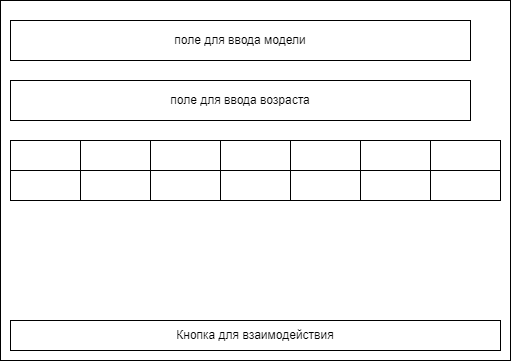
\includegraphics[width=0.55\textwidth]{maket}
    \caption{Макет экранной формы}
    \label{f:maket}
\end{figure}

Рассмотрим алгоритм работы модуля. Схема алгоритма представлена на рисунке~\ref{f:neuro-alg}.

\begin{figure}[h!]
    \centering
    \vspace{\toppaddingoffigure}
    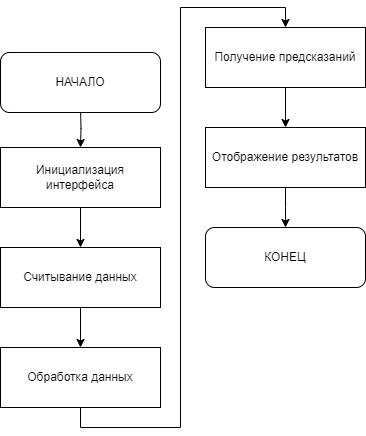
\includegraphics[width=0.45\textwidth]{neuro-alg}
    \caption{Алгоритм модуля}
    \label{f:neuro-alg}
\end{figure}

Рассмотрим алгоритм подробнее:
\begin{enumerate}
    \item  инициализация интерфейса. Модуль создает графический интерфейс. Он состоит из окна, содержащего поля для ввода модели и возраста, кнопки для выполнения предсказания и таблицы для отображения результатов;
    \item  считывание данных. Пользователь вводит данные в поля "Модель" и "Возраст";
    \item  обработка введенных данных. Данные из полей ввода предварительно обрабатываются таким же образом, как и обрабатывались данные, использующиеся для обучения нейронной сети;
    \item  получение предсказаний. Введенные данные (модель и возраст) передаются в обученную модель для выполнения предсказания интересов. Результаты предсказаний возвращаются в виде вероятностей принадлежности к каждой из категорий интересов;
    \item  отображение результатов. После получения результатов предсказаний, проценты принадлежности к каждой категории интересов отображаются в таблице. Каждый столбец таблицы соответствует одной из категорий интересов;
    \item  завершение работы интерфейса. После завершения работы с интерфейсом пользователь может закрыть окно, нажав на кнопку закрытия или продолжить работу;
\end{enumerate}


\section*{Выводы}

В данном разделе был рассмотрен процесс проектирования разрабатываемого модуля. Будет определен функционал и особенности. Кроме того, были разработаны алгоритмы функционирования, а также структура нейросети и самого модуля в целом.



